\documentclass{article}


% if you need to pass options to natbib, use, e.g.:
%     \PassOptionsToPackage{numbers, compress}{natbib}
% before loading neurips_2020

% ready for submission
% \usepackage{neurips_2020}

% to compile a preprint version, e.g., for submission to arXiv, add add the
% [preprint] option:
     \usepackage[preprint]{neurips_2020}

% to compile a camera-ready version, add the [final] option, e.g.:
 %    \usepackage[final]{neurips_2020}

% to avoid loading the natbib package, add option nonatbib:
%     \usepackage[nonatbib]{neurips_2020}

\usepackage[utf8]{inputenc} % allow utf-8 input
\usepackage[T1]{fontenc}    % use 8-bit T1 fonts
\usepackage{hyperref}       % hyperlinks
\usepackage{url}            % simple URL typesetting
\usepackage{booktabs}       % professional-quality tables
\usepackage{amsfonts}       % blackboard math symbols
\usepackage{nicefrac}       % compact symbols for 1/2, etc.
\usepackage{microtype}      % microtypography
\usepackage{graphicx}

\usepackage{booktabs, floatrow, makecell}
\floatsetup{floatrowsep=qquad}

\title{Consumer ABS (Name WIP)}

% The \author macro works with any number of authors. There are two commands
% used to separate the names and addresses of multiple authors: \And and \AND.
%
% Using \And between authors leaves it to LaTeX to determine where to break the
% lines. Using \AND forces a line break at that point. So, if LaTeX puts 3 of 4
% authors names on the first line, and the last on the second line, try using
% \AND instead of \And before the third author name.

\author{%

  James T. Bishop \\
  Department of Computer Science \\
  Boston University \\
  Boston, MA 02215 \\
  \texttt{jtbishop@bu.edu}
  % examples of more authors
  % \And
  % Coauthor \\
  % Affiliation \\
  % Address \\
  % \texttt{email} \\
  % \AND
  % Coauthor \\
  % Affiliation \\
  % Address \\
  % \texttt{email} \\
  % \And
  % Coauthor \\
  % Affiliation \\
  % Address \\
  % \texttt{email} \\
  % \And
  % Coauthor \\
  % Affiliation \\
  % Address \\
  % \texttt{email} \\
}

\begin{document}

\maketitle

\begin{abstract}
  This paper explores statistical relationships in Consumer Asset Backed Securities including the pricing of individual securities and probability of prepayment or default. As with Mortgage-Backed Securities, the largest risk an investor in Consumer ABS faces is prepayment risk. Identifying relevant factors to accurately quantify this risk is paramount to extracting value from the Consumer ABS market. 
\end{abstract}


\section*{Introduction}
Asset Backed Securities (ABS) are a class of financial structured product that pool together cash flow generating assets and payout that cash to the securities' holders. Consumer ABS are a category of ABS where the underlying asset pools come from credit card loans, student loans, auto loans, or specific merchant loans like Affirm or Afterpay. 

What makes Consumer ABS specifically interesting is how underdeveloped the market is, even relative to the rest of the ABS market or rest of the structured product market. Of the \$9.2 trillion strucutured products market, non-mortgage ABS comprised \$1.3 trillion, with consumer ABS making up about \$500 billion of this \citation{guggenheimABS}. 

\begin{figure}[h]
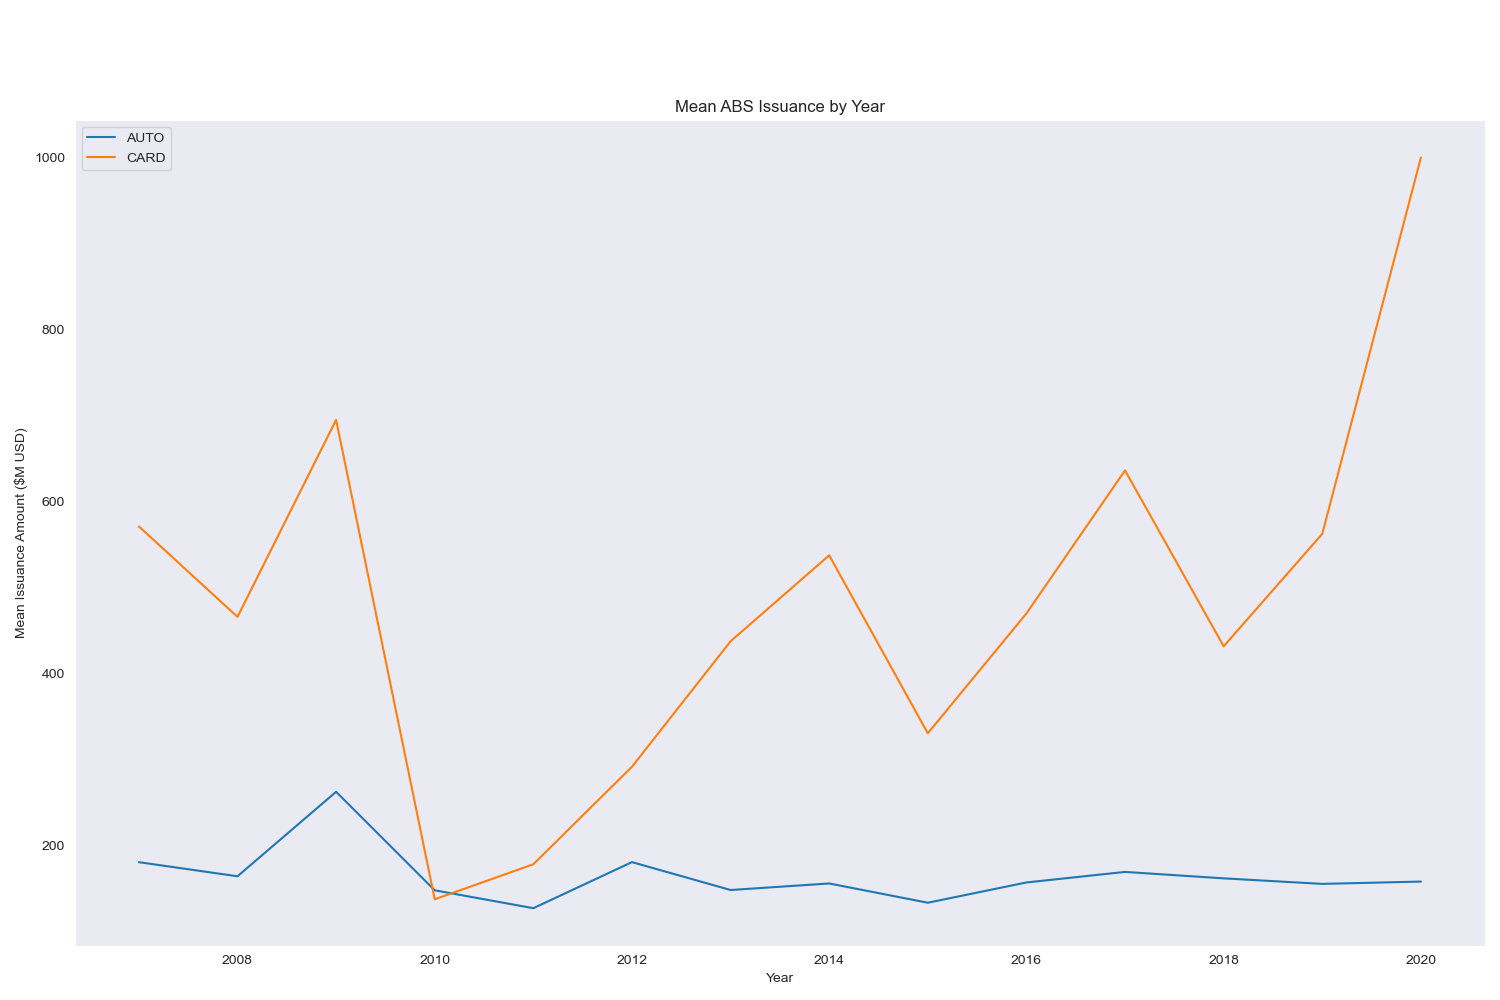
\includegraphics[scale=0.3]{meanIssuanceByYear}
\centering
\label{fig:meanABSIssuance}
\caption{Mean Auto and Card ABS Issuance}
\end{figure}

Pricing these securities is difficult for a few reasons. First, while many of these securities trade frequently, there is less transparency than in equity and other fixed income markets. Many consumer ABS deals don't have public information available, and even those that do aren't necessarily part of FINRA's Trade Reporting and Compliance Engine (TRACE), which functions to report trade data similar to what's available to the general public on stock trades. However, this data isn't typically available to retail investors because of a paywall. 

Second, most retail investors can't trade consumer ABS through their broker. This means fewer market participants and, as a result, more mispricings. 

Finally, ABS are complex products. Modeling their cash flows, prepayment and credit risk, and volatility is difficult, even if one assumes a perfectly efficient market. Due to this, there's a lower level of consistency in price determination between market makers (e.g. banks) which also makes price determination difficult. 

The goal of this project is to act as a primer on using modern data science methods to explore the ABS market and make ballpark price estimations.

\section*{Data}
Data was gathered through Boston University's Bloomberg Terminal subscription as well as the Federal Reserve of St. Louis (FRED) online database. 

From Bloomberg, the SRCH <GO> function was used to screen for public ABS deals (i.e. ABS issuances involving publicly traded companies) transacted in US dollars and with collateral in the US. Later, the SRCH <GO> function was also used to find the TRACE eligible subset of those deals. Additionally, individual bond prices for 20 bonds was gathered along with collateral for those bonds. The pricing data was gathered on a daily frequency while the collateral data was gathered at monthly frequency. 

From FRED, historic yields for the 1, 2, 3, 5, 7, 10, 20, and 30 year treasuries was pulled on a monthly basis. 

For data maps, see appendix.  

\section*{Implementation}
To start, I explored the data gathered using SECF <GO> and examined year over year mean issuance by ABS category, distribution of issuances by coupon type within each group and number and average dollar amount of each issuance by coupon type. Next, I removed non-TRACE eligible bonds from my dataset and looked at a correlation matrix of the remaining securities' features \ref{fig:TRACECorrelation}. I then used K-Means clustering with 10 clusters to find 10 general classes of TRACE eligible bonds, based on available features. From here, I took note of the 10 cluster centers and randomly selected one other security from a cluster. I used these 20 TRACE eligible bonds later for pricing and collateral. I made this decision since there was no feasible way for me to fetch data on a massive bond universe given the data restrictions imposed by Boston University's Bloomberg subscription. 

Following exploration, I made loader objects to load in my various data sources. These are all in the \texttt{preprocessing.py} file. I then began to look at ways to predict prepayments on the bonds in the TRACE Eligible dataset. \ref{TRACEEligible} I included all feature columns except "Is Mortgage Paid Off", "Next Call Date", "WAC", "Current WAL", and "Amt Out" because "Is Mortgage Paid Off" is our target variable, and the remaining variables' conditional distributions would reveal very clearly whether or not a security had been prepaid. I then took use One Hot Encoding on the categorical features, made the date features Gregorian ordinal values, and used a label encoder on the remaining columns. 

I trained kNN, SVM, Gaussian Process, Decision Tree, Random Forest Classifier, Multilayer Perceptron, AdaBoost, Naive Bayes, and Quadratic Discriminant classifiers on 80\% of the data and tested them on 20\%. Results will be discussed in \ref{Results}. 

Following the classification task, I attempted to use Generalized Least Squares to predict monthly returns on the 20 securities mentioned earlier. I merged the price and collateral DataFrames with historic treasury yields. Since this was timeseries data, I then lagged the exogenous variables by 1 timestep. 


\section*{Results} 
\label{Results}

In classification, I considered RMSE, accuracy, recall, and F1 Score and found that a Decision Tree with a max depth of 14 performed best: 

\begin{verbatim}
Test: RMSE of Pipeline(steps=[('decisiontreeclassifier',
                 DecisionTreeClassifier(max_depth=14))]) is 0.139
              precision    recall  f1-score   support

           0       0.99      0.99      0.99       178
           1       0.93      0.93      0.93        29

    accuracy                           0.98       207
   macro avg       0.96      0.96      0.96       207
weighted avg       0.98      0.98      0.98       207
\end{verbatim}

In the return prediction task, results for Auto and Consumer loans looked like this: 

\begin{verbatim}
Results for CARMX 2018-1 A4
                                 GLS Regression Results                                
=======================================================================================
Dep. Variable:                  Price   R-squared (uncentered):                   0.829
Model:                            GLS   Adj. R-squared (uncentered):              0.712
Method:                 Least Squares   F-statistic:                              7.076
Date:                Fri, 27 Nov 2020   Prob (F-statistic):                    8.33e-05
Time:                        09:44:51   Log-Likelihood:                          179.65
No. Observations:                  32   AIC:                                     -333.3
Df Residuals:                      19   BIC:                                     -314.3
Df Model:                          13                                                  
Covariance Type:            nonrobust                                                  
==============================================================================
                 coef    std err          t      P>|t|      [0.025      0.975]
------------------------------------------------------------------------------
WAC           -0.0247      0.016     -1.564      0.134      -0.058       0.008
WAM            0.0027      0.001      2.775      0.012       0.001       0.005
WALA           0.0029      0.002      1.331      0.199      -0.002       0.008
Balance       1.9e-12   4.49e-11      0.042      0.967    -9.2e-11    9.58e-11
Principal   -8.48e-11   1.64e-10     -0.519      0.610   -4.27e-10    2.57e-10
DGS1           0.0020      0.011      0.178      0.861      -0.022       0.026
DGS2          -0.0182      0.055     -0.333      0.742      -0.133       0.096
DGS3           0.0095      0.069      0.137      0.892      -0.135       0.154
DGS5           0.0032      0.041      0.077      0.940      -0.083       0.089
DGS7          -0.0159      0.033     -0.483      0.635      -0.085       0.053
DGS10          0.0405      0.024      1.690      0.107      -0.010       0.091
DGS20         -0.0339      0.030     -1.139      0.269      -0.096       0.028
DGS30          0.0139      0.022      0.624      0.540      -0.033       0.060
==============================================================================
Omnibus:                        1.544   Durbin-Watson:                   2.084
Prob(Omnibus):                  0.462   Jarque-Bera (JB):                1.018
Skew:                          -0.437   Prob(JB):                        0.601
Kurtosis:                       2.987   Cond. No.                     4.15e+11
==============================================================================


\end{verbatim}

Results for Card loans looked like: 

\begin{verbatim}
Results for AMXCA 2018-3 A
                                 GLS Regression Results                                
=======================================================================================
Dep. Variable:                  Price   R-squared (uncentered):                   0.804
Model:                            GLS   Adj. R-squared (uncentered):              0.544
Method:                 Least Squares   F-statistic:                              3.084
Date:                Fri, 27 Nov 2020   Prob (F-statistic):                      0.0271
Time:                        09:44:51   Log-Likelihood:                          181.82
No. Observations:                  28   AIC:                                     -331.6
Df Residuals:                      12   BIC:                                     -310.3
Df Model:                          16                                                  
Covariance Type:            nonrobust                                                  
==================================================================================
                     coef    std err          t      P>|t|      [0.025      0.975]
----------------------------------------------------------------------------------
ExcessSpread3M    -0.0004      0.001     -0.566      0.582      -0.002       0.001
ExcessSpread1M  3.192e-05      0.001      0.053      0.959      -0.001       0.001
Mth Pay Rate    2.215e-05      0.000      0.141      0.891      -0.000       0.000
Port Yld           0.0002      0.000      0.473      0.645      -0.001       0.001
Chg Offs       -7.907e-05      0.001     -0.061      0.952      -0.003       0.003
30                -0.0128      0.011     -1.206      0.251      -0.036       0.010
60                 0.0036      0.016      0.229      0.822      -0.031       0.038
del90Plus          0.0063      0.008      0.825      0.426      -0.010       0.023
DGS1               0.0022      0.009      0.244      0.811      -0.018       0.022
DGS2              -0.0262      0.037     -0.701      0.497      -0.108       0.055
DGS3               0.0288      0.050      0.576      0.575      -0.080       0.138
DGS5               0.0130      0.027      0.476      0.643      -0.047       0.073
DGS7              -0.0217      0.031     -0.705      0.494      -0.089       0.045
DGS10              0.0002      0.021      0.009      0.993      -0.045       0.046
DGS20             -0.0015      0.019     -0.075      0.941      -0.044       0.041
DGS30              0.0054      0.021      0.262      0.798      -0.040       0.051
==============================================================================
Omnibus:                       14.666   Durbin-Watson:                   2.219
Prob(Omnibus):                  0.001   Jarque-Bera (JB):               26.520
Skew:                           0.924   Prob(JB):                     1.74e-06
Kurtosis:                       7.395   Cond. No.                     4.49e+04
==============================================================================


\end{verbatim}

Both sets of data showed statistical significance at at least the 5\% level, based on simultaneous hypothesis tests for the explanatory variables in the model. 

\section*{Challenges}
The biggest challenge in this project was data availability. Despite the cleanliness of data provided by Bloomberg, the amount of data with useful features was limited. It was impossible to pull a large universe of securities all at once, even in the screening phase which meant that there were approximately $1,000$ securities used in the classification task. Similarly, it was impossible to fetch a high volume of individual bond prices or collateral at once, and scripting was not an option which meant a small universe of securities for tasks using that data.

Another evident challenge is the complexity of ABS. For instance, the LIBOR Market Model (LMM) is a popular tool for pricing structured products, among other things. However, calibrating the model is a complex optimization process as is applying the model to data, particularly when the data available is low frequency and there isn't a lot available. 


 


\section*{Conclusion \& Takeaways}
The largest takeaway is that a Decision Tree Classifier is very well suited to the task of predicting whether a security has defaulted or not, given this dataset. Obviously, one key issue with this is that we haven't predicted when or how likely that default is, which means that it's difficult to quantify the risk associated with it. This is discussed in greater detail in \ref{Future Work}. 

This paper also provides a starting point for time series analysis of ABS prices. By looking at a small number of factors, relatively accurate predictions were able to be made. To really see the performance of the GLS model, however, backtesting would be required, which wasn't possible with the data available. This is also a source of future work. 

\section*{Future Work}
\label{Future Work}
I plan to gather incrementally more data and build a larger set of securities with collateral and pricing. In doing so, I'll be able to more produce results with a higher degree of certainty.

I also intend to examine price at issue data and gather text files of filing documents and news on companies issuing these debt securities to see whether or not sentiment analysis has a place in accurately pricing initial offerings.

Further, I am working on implementing LMM. The difficulty lies in the frequency of data I have available because typically the model is used on extremely high frequency data, e.g. 1 minute intervals rather than days or months.

As mentioned earlier, the Decision Tree Classifier doesn't answer "How risky is this security?" or "When will we likeliest see prepayments occur?". To do so requires a more complex model, and is something I plan to explore in the future, hopefully using properties of the LMM model. 
\section*{Appendix}
\begin{table}[h]
  \small\centering
  \begin{floatrow}
    \ttabbox{ \caption{ABS Trace Issuance Datasets} \label{ABSTrace}}
   {\begin{tabular}{lll}
\toprule
Label &               Type  & Description \\
\midrule
Amt Out                    &         float64 & Amount outstanding (USD) \\
BBG Composite              &          object & Bloomberg Composite credit rating \\
CUSIP                      &          object & \\
Cpn                        &         float64 & Coupon (\%) \\
Current WAL                &         float64 & Current Weighted Average Life \\
Day Count                  &          object & Day count convention (30/360, 30/365, or Actual)\\
Delinquency Rate 60+ Days  &         float64 & \\
Delinquency Rate 90+ Days  &         float64 & \\
Issue Date                 &  datetime64[ns] & \\
Issuer Name                &          object & \\
Maturity                   &  datetime64[ns] & \\
Mid Price                  &         float64 & Mid price between bid and ask price \\
Mortgage Original Amount   &           int64 & \\
Next Call Date             &  datetime64[ns] & Only applicable to callable bonds \\
Next Coupon Date           &  datetime64[ns] & \\
Original Maximum Loan Size &         float64 & Size of largest loan in the pool at issue \\
Price at Issue             &         float64 & \\
Security Name              &          object & \\
Ticker                     &          object &\\
Category                   &          object & CARD, AUTO, or CONSUMER \\
Original WAL               &         float64 & Original Weighted Average Life \\
isCallable                 &         float64 & \\
\bottomrule
\end{tabular}}
  \end{floatrow}
\end{table}

\begin{table}[h]
  \small\centering
  \begin{floatrow}
    \ttabbox{ \caption{TRACE Eligible Loans Dataset} \label{TRACEEligible}}
   {\begin{tabular}{lll}
\toprule
Label &               Type  & Description \\
\midrule
CUSIP                     &          object & \\
Security Name             &          object & \\
Mortgage Original Amount  &         float64 & \\
Cpn                       &         float64 & Coupon (\%)\\
Current WAL               &         float64 & \\
Amt Out                   &         float64 & Amount outstanding (USD) \\
BBG Composite             &          object & Bloomberg Composite credit rating \\
Day Count                 &          object &  Day count convention (30/360, 30/365, or Actual) \\
Delinquency Rate 60+ Days &         float64 & \\
Delinquency Rate 90+ Days &         float64 & \\
Is Mortgage Paid Off      &           int64 & \\
Issue Date                &  datetime64[ns] & \\
Maturity                  &  datetime64[ns] & \\
Next Call Date            &  datetime64[ns] & \\
Ticker                    &          object & \\
Price at Issue            &         float64 & \\
Benchmark Spread at Issue &         float64 & Spread to the benchmark rate at issue \\
PSA Since Issuance        &         float64 & Public Securities Association prepayment calculation \\
WAC                       &         float64 & Weighted Average Coupon \\
Category                  &          object & CARD, AUTO, or CONSUMER \\
isCallable                &         float64 & \\
Original WAL              &         float64 & Original Weighted Average Life \\
\bottomrule
\end{tabular}}
  \end{floatrow}
\end{table}

\begin{table}[h]
  \small\centering
  \begin{floatrow}
    \ttabbox{ \caption{Collateral for Credit Card ABS} \label{CreditCollat}}
   {\begin{tabular}{lll}
\toprule
Label &               Type  & Description \\
\midrule
ExcessSpread3M &  float64 \\
ExcessSpread1M &  float64 \\
Mth Pay Rate   &  float64 \\
Port Yld       &  float64 \\
Chg Offs       &  float64 \\
30             &  float64 & 30 day delinquency rate \\
60             &  float64 & 60 day delinquency rate\\
del90Plus      &  float64 & 90 day delinquency rate\\
\bottomrule
\end{tabular}}
  \end{floatrow}
\end{table}

\begin{table}[h]
  \small\centering
  \begin{floatrow}
    \ttabbox{ \caption{Collateral for Auto and Consumer ABS} \label{OtherCollat}}
   {\begin{tabular}{lll}
\toprule
Label &               Type  & Description \\
\midrule
WAC       &  float64 & Weighted Average Coupon \\
WAM       &    int64 & Weighted Average Maturity \\
WALA      &    int64 & Weighted Average Loan Age \\
Balance   &    int64 & \\
Principal &  float64 & \\
\bottomrule
\end{tabular}}
  \end{floatrow}
\end{table}

\begin{figure}
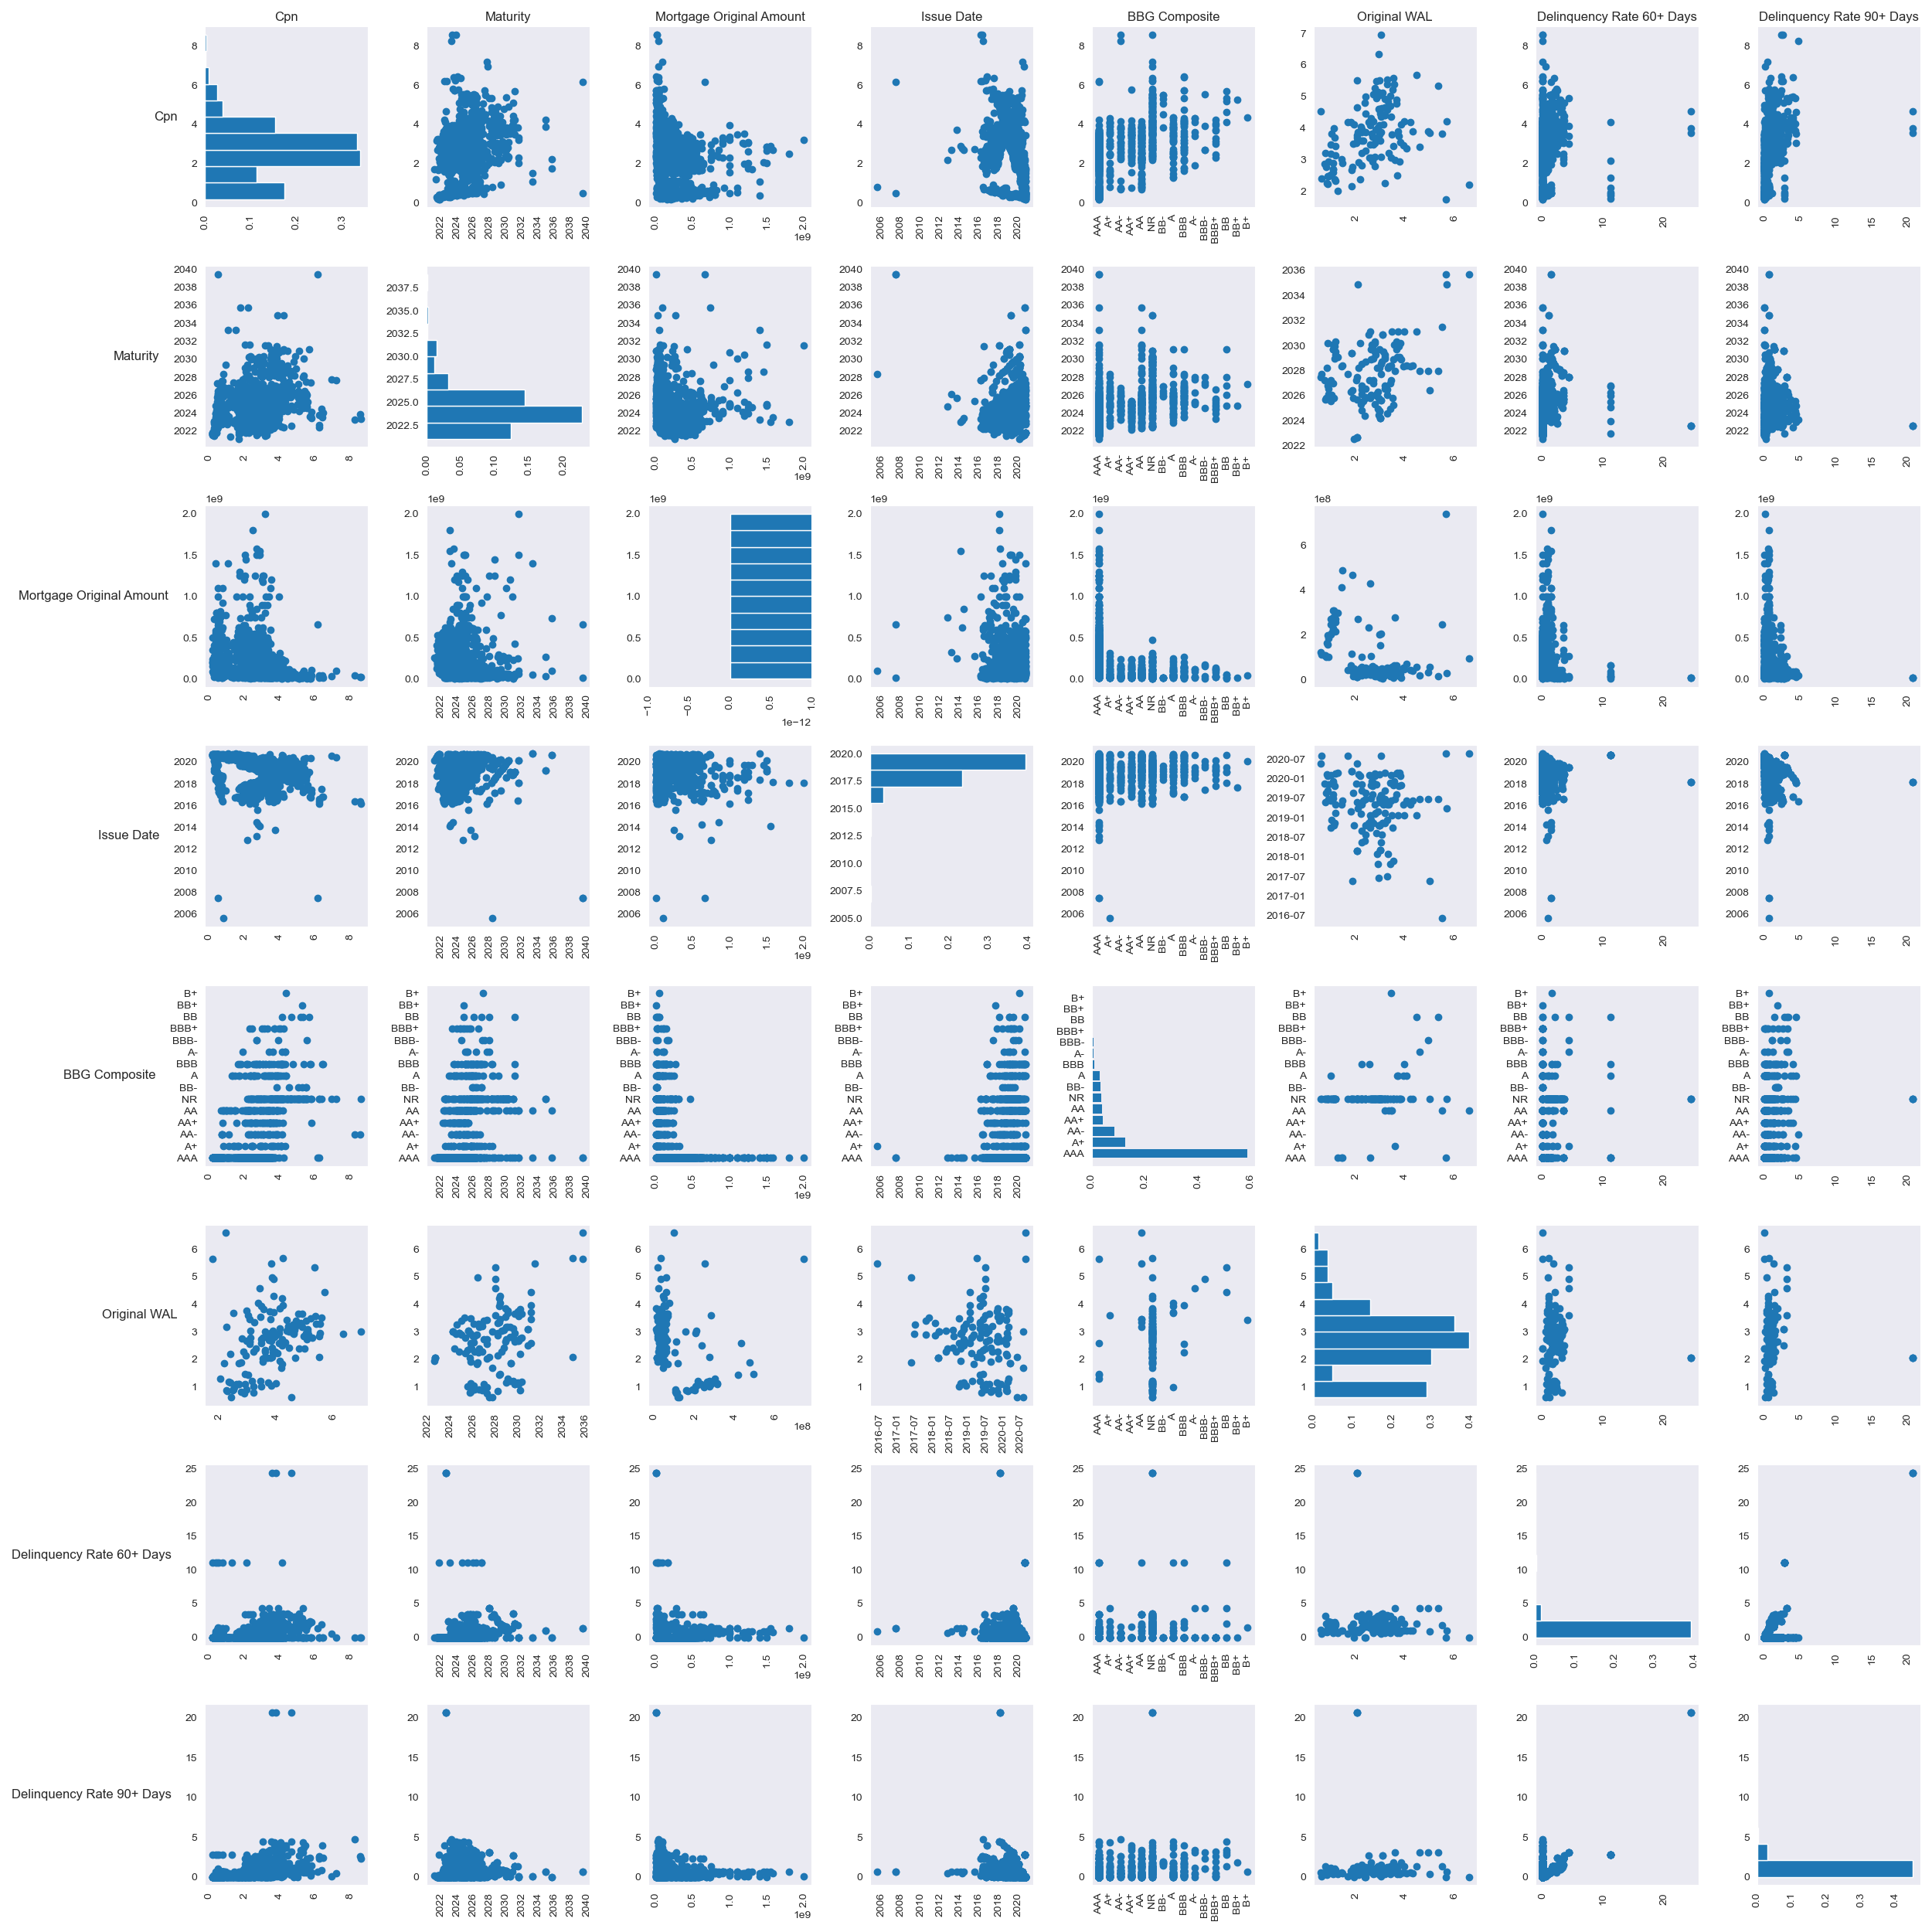
\includegraphics[scale=0.2]{TRACECorrelationMatrix}
\centering
\label{fig:TRACECorrelation}
\caption{Correlation Matrix of TRACE Eligible Bonds}
\end{figure}


\newpage

\bibliography{ref}
\bibliographystyle{chicago}

\end{document}
